%!TEX root = ../main.tex
%%%%%%%%%%%%%%%%%%%%%%%%%%%%%%%%%%
% Links:
%
% Difficulty: Companies: 
%%%%%%%%%%%%%%%%%%%%%%%%%%%%%%%%%%

\chapter{Largest square in a binary matrix}
% type of problem why can be useful in real life (image segmentation) dynamic programming
\label{ch:square_in_matrix}
\section*{Introduction}
Imagine you are given a black and white image represented as a boolean matrix of size $N\times M$
where $0$ and $1$ in the matrix correspond to a black and white pixel respectively. Such kind of
image are less uncommon that might be thought at first because they are often the output of digital
image processing algorithms such as masking or thresholding. Further analyzing this kind of images
often requires to identify homogeneous portions of the image. The problem described in this chapter
deals with a simple type of image processing algorithm that involves determining the size of the
largest square area of white pixel of a binary bitmap. We will walk through a number of solutions,
starting from a naive brute-force one, to a more sophisticated, more complex and definitely more
efficine one.
 

\section{Problem statement}
\begin{exercise}
Given a 2D boolean matrix, return the area of the largest square containing only one cells.
	\begin{example}
		\hfill \\
		Given the following matrix the function returns $9$. The largest square has side lenght of
		$3$ and the coordinate of the top-left corner are $(2,1)$. Cells belonging to the largest
		square are highlighted.

		\begin{tabular}{|l|l|l|l|l|}
		\hline
		0 & 0                                  & 1                                  & 1 & 1 \\
		\hline
		0 & 0                                  & 1                                  & 1 & 0 \\
		\hline
		0 & \cellcolor[HTML]{32CB00}\textbf{1} & \cellcolor[HTML]{32CB00}\textbf{1} &
		\cellcolor[HTML]{32CB00}\textbf{1} & 0 \\ \hline
		1 & \cellcolor[HTML]{32CB00}\textbf{1} & \cellcolor[HTML]{32CB00}\textbf{1} &
		\cellcolor[HTML]{32CB00}\textbf{1} & 0 \\ \hline
		1 & \cellcolor[HTML]{32CB00}\textbf{1} & \cellcolor[HTML]{32CB00}\textbf{1} &
		\cellcolor[HTML]{32CB00}\textbf{1} & 0 \\ \hline
		\end{tabular}
		
	\end{example}

	\begin{example}
		\hfill \\
		Given the following matrix the function returns $4$. The side of the largest square is $2$
		and the top-left coordinates are $(2,2)$. Cells belonging to the largest square are
		highlighted.
		\begin{tabular}{|l|l|l|l|l|}
		\hline
		1 & 0 & 1                                  & 0                                  & 0 \\
		\hline
		1 & 0 & \cellcolor[HTML]{32CB00}\textbf{1} & \cellcolor[HTML]{32CB00}\textbf{1} & 1 \\
		\hline
		1 & 1 & \cellcolor[HTML]{32CB00}\textbf{1} & \cellcolor[HTML]{32CB00}\textbf{1} & 1 \\
		\hline
		1 & 0 & 0                                  & 1                                  & 0 \\
		\hline
\end{tabular}

	\end{example}

\end{exercise}


\section{Discussion}
\label{square_in_matrix:sec:discussion}
In the next section we will analyze a number of possible approaches to this problem. We start by
looking at a few brute-force approaches so to then move towards more elaborate and more time and
space efficient dynamic programming solutions

\subsubsection{Brute-force - Incremental side}
\label{square_in_matrix:sec:incremental_side}
The first brute-force approach consists of trying to find the largest square made entirely of
set (i.e. holding a value of $1$) cell by visiting each set cell and by treating it as if it was the top-left corner
of a square. Because calculating the largest square having that cell as top-left corner is easy the
answer is just the largest value calculated over all the set cells in the matrix. In order to find out
what the value of the largest square having cell $(x,y)$ as top-left corner we can
try build squares of incrementally larger sides around it, starting from side lenght $1$.
At first we try to build a square of size $1$. If that is possible we try size $2$, then $3$, and so on, until it is impossible or we hit the boundaries of the matrix.
The answer for the cell $(x,y)$ is the last value for a side for which we were able to construct a square.

This approach is clearly correct because eventually we find all possible squares in the matrix, and has a
complexity of (assuming, with no loss in generality, $N \leq M$) $O(N^4M)$. This is because there are $O(NM)$ possible starting point for
a square, $O(N)$ possible values for a side of a square and checking whether a square is
valid costs $O(N^2)$ (all cells in the square needs to be checked). A possible implementation of such idea is
shown in the Listing \ref{list:square_in_matrix:bruteforce1}.


\lstinputlisting[language=c++, caption={Brute force soltuion solution to the "largest square in matrix" problem using incremental side approach.},label=list:square_in_matrix:bruteforce1]{sources/square_in_matrix/square_in_matrix_solution1.cpp}


\subsubsection{Brute-force improved}
The idea presented in the Section \ref{square_in_matrix:sec:incremental_side}
can be significantly improved by noticing that is it really not necessary to
check, for every cell, squares of all possible side lenghts.
The idea is that we can walk diagonally (towards the bottom-right cell)
from $(x,y)$ (by incrementing the both $x$ and $y$). For every step $i$ we take,
we check whether all the elements to the left of $(x+i, y+i)$  and to the
right of  $y$ are set, and also whether all the cells in the columns above
$(x+i, y+i)$ and below the cell $(x,y+i)$ are set. If both conditions are true
it means that we can construct a square of side $k$. We can then proceed to
check the next $k$ until a $0$ is found or the limit of the matrix are hit. If
we were able to perform $t$ diagonal steps,
it means we have found out that the largest square having $(i,j)$ as top-left
corner has an area of $t^2$. The final answer is the largest value we calculated
this way across all cell that are set. See Figure \ref{fig:square_in_matrix:squa_matrix_incremental}.


\begin{figure}
	\centering
	\label{fig:square_in_matrix:squa_matrix_incremental}
	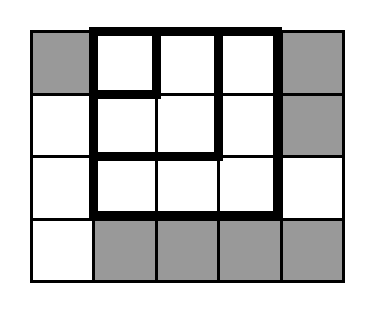
\includegraphics[width=\textwidth/2]{sources/square_in_matrix/images/squa_matrix_incremental}
	\caption{ddddddddddddddddddd }
\end{figure}

The time complexity of this approach is lower than the previous case i.e. $N^3M$
because as in the solution shown in Section
\ref{square_in_matrix:sec:incremental_side} there are $NM$ potential top-left
corner for a square and for each of them $O(N)$ diagonal steps. Each diagonal
steps costs $O(N)$ as in the worst case we must only check one entire row and
column. 


\lstinputlisting[language=c++, caption={Sample Caption},label=list:square_in_matrix]{sources/square_in_matrix/square_in_matrix_solution1.cpp}



look for 
\begin{itemize}
	 \item count the number of consecutive ones in the right direction starting at $(i,j)$. In other
	 words how many steps we can take from $(i,j)$ in the right direction  before we either find a
	 $0$ or hit the limit of the matrix? 
	 \item count the number of consecutive ones in the downwards direction starting at $(i,j)$. In
	 other words how many steps we can take from $(i,j)$ in the down direction before we either find
	 a $0$ or hit the limit of the matrix? 
\end{itemize}
The minimum between this number ($s_{i,j}$) will give us an indication of the biggest square that
can be created from $(i,j)$. We can then proceed and check if all the cells in the square having as
top-left corner $(i,j)$ and down-right corner $(i+s_{i,j},j+s_{i,j})$ are all set to $1$. If that is
the case we have found a square of size $s_{i,j}$ starting at $(i,j)$. 

Among all squares, we shall return the largest one. 

\begin{figure}
	\centering
	\label{fig:square_in_matrix:square_matrix_diagonal}
	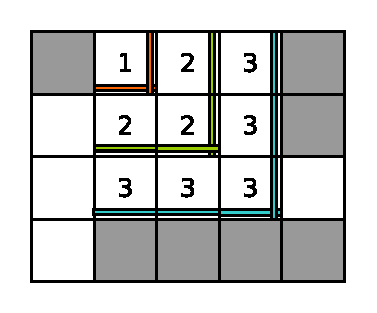
\includegraphics[]{sources/square_in_matrix/images/square_matrix_diagonal}
	\caption{ddddddddddddddddddd }
\end{figure}


\subsubsection{Brute-force 1}


